\chapter{Tribler functionality}
% Desktop version
% Trible intro, what is it (read thesis independently)
% explain what has been done to fix attack-reselience, VOD, self-organising, etc...


\section{Video-on-demand}

% digitaler, vod komt meer voor, videotheek was het al, youtube nu ook, netflix
% mensen bepalen zelf wanneer ze wat zien, geen tv broadcast
% ook streaming, no waiting
% Tribler doet dit ook, plus ...
% verschil is...
% aangeven dat je anoniem wilt downloaden is nieuw
% youtube kan dat niet, geen hoofdfunctionaliteit

Tribler introduces a server-less video-sharing platform with privacy enhancing technologies that provides a Youtube-like social media experience.
Video-on-demand means that users can simply click and play videos in a streaming fashion, so without waiting for the entire video to be present on the device. %dit is streaming, geen vod
You can search from within the application and browse for videos in channels rated automatically by popularity.
Simply clicking on a video and watching it while streaming is supported via the BitTorrent-aware Tribler video server and integrated video player VLC.


\section{Self-organizing}

The BitTorrent protocol is used to download and upload the content.
A BitTorrent swarm can use the "distributed sloppy hash table" (DHT) of a specific torrent to discover peers and gather meta-information.
Also part of the DHT protocol is the self-organizing behavior of maintaining a routing table of known good nodes.
Tribler uses these features to coordinate the exchange of videos and meta-data fully automatically.
Users do not have to manage any files or configuration manually at all to be active on the platform.


\section{Autonomous operation}

New content discovery can be discovered automatically via a "Channel"-community that users can subscribe to.
Communities are network overlays used by Tribler to offer functionality like search, add, remove and comment on content.
To discover all channels in existence Tribler is subscribed to the so called "AllChannel"-community and "Search"-community by default.
These are used to exchange information about what channels and torrents are out there and who likes them and knows about them.
Each channel has its own community that rules permissions and meta-data of content.
These communities operate autonomously and are transparent to the user, who only sees channels and search results show up in the GUI.


\section{Attack-resilience}

The server-less technique of Tribler is resistant to large scale monitoring and censorship, because there is no central point that can be controlled to gather or block information easily.
To monitor or censor the network effectively on a large scale you need control of a significant number of the communication links.
Censorship does not have an effect if the majority of users does not cooperate with the censor.
The beauty of a fully distributed design is that communicating directly between peers, or via a local network, works without the need for external communication links.
This is why the server-less technique of Tribler is resistant to Internet kill-switches as well because, even if the attacker can block all communication-links, users can always connect off-grid.
Such kill-switches are typically deployed for the purpose of censorship, but won't stop a connectible device, like a laptop, from physically moving.
No network infrastructure is required for viral spreading of the entire video platform.

These properties will ensure social media with resilience against Internet kill switches, natural disasters and censorship.


\section{Anonymity}

Tribler can protect the privacy of users by hiding their identity.
To connect to others on the network anonymous connections are created on behalf of downloaders and uploaders.
By routing the network traffic over a circuit of multiple hops it becomes difficult to trace the origin and destination.
This way the privacy of users remains protected while they actively participate on the platform

\begin{figure}[h]
	\centering
	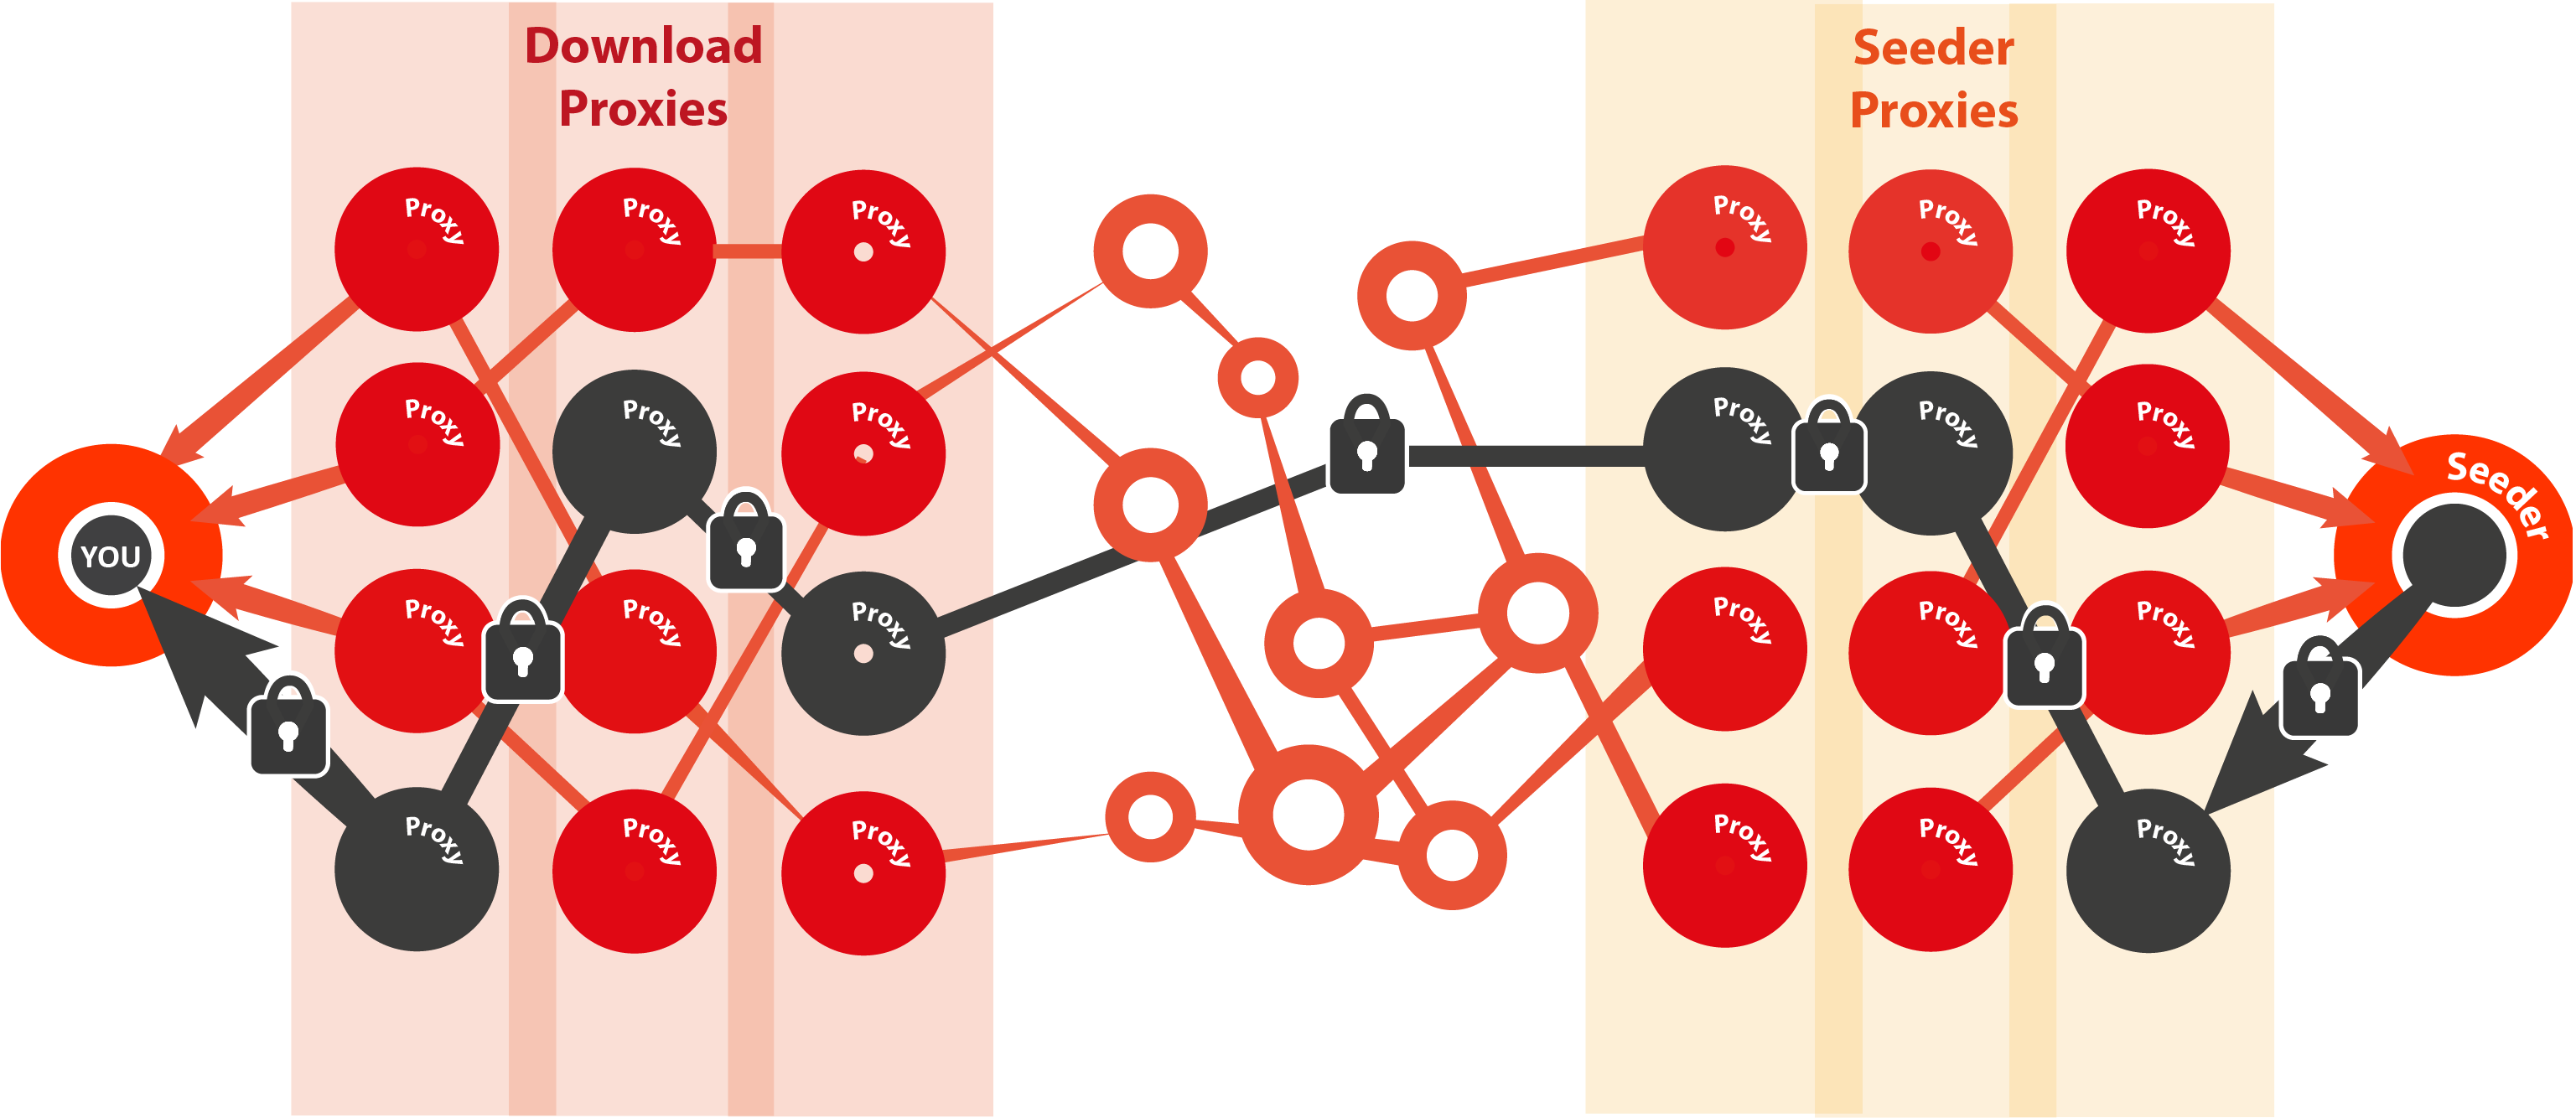
\includegraphics[width=\textwidth]{anonymity_proxies}
	\caption{Anonymity via proxies}
	\label{fig:anonymity_proxies}
\end{figure}

Multiple encrypted tunnels are layered such that every consecutive tunnel from the initiator to a relay is going through the previous tunnel.
Every relay works on behalf of its predecessor so no relay knows the identity of the initiator save for the first relay.
Since all communication is properly encrypted no relay can perform a successful man-in-the-middle attack.

This is similar to how Tor works, except Tribler uses UDP rather than TCP for performance reasons.

The capability of hiding your identity is greatly advantageous to the user if his or her human rights are violated, like free speech.

However, this privacy feature requires a lot more bandwidth of the network than without anonymity: a ratio of 13 GB for every anonymous 1 GB of data.
Since bandwidth is limited and transitory it can be beneficial to exchange unused bandwidth for a promise of bandwidth in the future, or another reward.
The research group behind Tribler is currently building a fully decentralized accounting system and open exchange market using block-chain technology with the purpose of building trust on-line and creating the Internet of Money.



